\documentclass[a4paper,ngerman,12pt]{scrartcl}

\usepackage[utf8]{inputenc}

\usepackage[ngerman]{babel}

\usepackage{amsmath,amsthm,amssymb,stmaryrd,color,graphicx,mathtools}
\usepackage{array}
\usepackage[all]{xy}

\usepackage{shadethm}

\usepackage[protrusion=true,expansion=true]{microtype}

\usepackage{minted}
\setminted{linenos}

\usepackage[T1]{fontenc}
\usepackage{libertine}

\usepackage{hyperref}

\setlength{\shadeboxsep}{6pt}
\setlength{\shadeleftshift}{-\shadeboxsep}
\setlength{\shaderightshift}{-\shadeboxsep}

\theoremstyle{definition}
\newtheorem{defn}{Definition}[section]
%\newtheorem{defn}{Definition}[section]
\newtheorem{ex}[defn]{Beispiel}
\newtheorem{motto}[defn]{Motto}

\theoremstyle{plain}

\newtheorem{defnprop}[defn]{Definition/Proposition}
\newtheorem{prop}[defn]{Proposition}
\newtheorem{fact}[defn]{Fakt}
\newtheorem{lemma}[defn]{Lemma}
\newtheorem{thm}[defn]{Satz}
\newtheorem{cor}[defn]{Korollar}

\theoremstyle{remark}
\newtheorem{rem}[defn]{Bemerkung}
\newtheorem{warning}[defn]{Warnung}

\clubpenalty=10000
\widowpenalty=10000
\displaywidowpenalty=10000

\newcommand{\RR}{\mathbb{R}}
\newcommand{\CC}{\mathbb{C}}
\newcommand{\DD}{\mathbb{R}[\varepsilon]/(\varepsilon^2)}
\newcommand{\defeq}{\vcentcolon=}

\begin{document}

\title{Automatic Differentiation}
\author{Ingo Blechschmidt}
\date{July 9th, 2015}
\maketitle

\section{What automatic differentiation achives}

Given code which implements a function~$x \mapsto f(x)$, automatic
differentiation gives us code which implements its derivative~$x \mapsto
f'(x)$. The code obtained this way is exactly the same as if we'd worked out
the derivative on paper.

The input code to automatic differentiation may contain arbitrary control
structures such as \emph{if} conditionals or \emph{while} loops. Therefore it
is applicable to a wide range of problems:

\begin{itemize}
\item The basic use case is to find the derivative of a function.
\item Assume that we're using Newton's method to solve a parameter-dependent
equation~$f(x,\theta) = 0$ for~$x$. We might be interested in how the
solution~$x(\theta)$ depends on~$\theta$. This is trivial with automatic
differentiation, we just feed it our Newton code.
\item Assume that we're solving some parameter-dependent ordinary differential
equation. We are interested in the dependence of the solution (at the final
time, say) on the parameter. For this, we just hand our differential equation
solving code to automatic differentiation.
\end{itemize}

Automatic differentiation is totally unlike \emph{numerical
differentiation}. With numerical differentiation, we approximate~$f'(x)$ by
some difference quotient like
\[ \frac{f(x + h) - f(x)}{h} \qquad\text{or}\qquad
  \frac{f(x + h) - f(x - h)}{2h}. \]
This approach faces severe problems: If~$h$ is large, the quotient won't be a
good approximation to the true derivative. Instead, it will give the slope of
some unrelated secant. If~$h$ is small, the approximation will be good in
theory. But practically, with floating-point arithmetic, a huge loss of
precision may occur, since we are subtracting two nearly equal numbers.

Automatic differentiation is also unlike \emph{symbolic differentiation},
which operates on the level of \emph{terms}. Symbolic differentiation is useful
if our goal is to obtain \emph{formulas} for various quantities, but it isn't
particularly suited for efficient evaluation to floating-point numbers.


\section{The basic idea of automatic differentiation}

To grasp the basic idea of automatic differentiation, assume that there exists
a magical number~$\varepsilon$ such that~$\varepsilon^2 = 0$. This
number~$\varepsilon$ should not itself be zero, as else we couldn't extract any
meaningful information from calculations with~$\varepsilon$.

The set of real numbers doesn't contain such a number. Nevertheless, watch:
\begin{align*}
  (x+\varepsilon)^2 &= x^2 + 2x\varepsilon + \varepsilon^2 = x^2 + 2x\varepsilon \\[0.6em]
  (x+\varepsilon)^3 &= x^3 + 3x^2\varepsilon + 3x\varepsilon^2 + \varepsilon^3 = x^3 + 3x^2\varepsilon \\[0.6em]
  \frac{1}{x+\varepsilon} &= \frac{x-\varepsilon}{(x+\varepsilon) \cdot
  (x-\varepsilon)} = \frac{x-\varepsilon}{x^2} = \frac{1}{x} - \frac{1}{x^2}
  \varepsilon
\end{align*}

So it appears that plugging in~$x + \varepsilon$ into a function~$f$ yields
\emph{the derivative~$f'(x)$ along with the function value~$f(x)$}, as the
coefficient of the magical number~$\varepsilon$.

We exploit this observation with automatic differentiation. To calculate the
derivative~$f'(x)$, given code for~$f(x)$, we feed the code with~$x +
\varepsilon$ and then extract the coefficient of~$\varepsilon$ from the result.
Of course, the given code didn't expect to be called with
magical~$\varepsilon$'s instead of ordinary floating-point numbers. But in a
language with operator overloading, there's no way for the code to prevent such
unusual evaluations. We discuss this in more detail below.


\section{A closer look: the dual numbers}

Recall how we construct the complex numbers~$\CC$ from the real numbers~$\RR$.
We define~$\CC \defeq \RR \times \RR$ and set
\begin{align*}
  (x,a) + (y,b) &\defeq (x+y, a+b), \\
  (x,a) \cdot (y,b) &\defeq (xy - ab, xb+ay).
\end{align*}
These formulas don't appear from nowhere. Instead, setting~$i \defeq (0,1)$,
they are precisely the formulas needed such that the identity~$i^2 = -1$
holds. Writing~$(x,a) = x + ai$, we call~$x$ the \emph{real part} and~$a$ the
\emph{imaginary part}.

In a similar way, we can construct the \emph{dual
numbers}~$\DD$. We
define~$\DD \defeq \RR \times \RR$ and set
\begin{align*}
  (x,a) + (y,b) &\defeq (x+y, a+b), \\
  (x,a) \cdot (y,b) &\defeq (xy, xb+ay).
\end{align*}
Again, these formulas can be motivated. We write~$\varepsilon \defeq (0,1)$
and~$x + a \varepsilon \defeq (x,a)$. Then these rules can be obtained by
formally expanding~$(x + a \varepsilon) + (y + b \varepsilon)$ respectively~$(x
+ a \varepsilon) \cdot (y + b \varepsilon)$ and imposing the
relation~$\varepsilon^2 = 0$.

It's easy to implement a data type of dual numbers in languages such as Haskell
or Python.

\begin{minted}{haskell}
-- Haskell
data D a = D a a deriving (Show,Eq)

instance (Num a) => Num (D a) where
    D x a + D y b  = D (x + y)         (a + b)
    D x a * D y b  = D (x * y)         (x * b + a * y)
    negate (D x a) = D (negate x)      (negate a)
    fromInteger n  = D (fromInteger n) 0
\end{minted}

If \mintinline{haskell}{f} is a function \mintinline{haskell}{(Num a) => a ->
a}, then evaluating \mintinline{haskell}{f (D x 1)} will yield
\mintinline{haskell}{D (f x) (f' x)}. A live example in the interactive Haskell
shell looks like this:

\begin{verbatim}> let f x = x^2
> f (D 5 1)
D 25 10
\end{verbatim}

We can also define a higher-order function which takes a function and returns
its derivative:

\begin{verbatim}> let diff f x = b where D y b = f (D x 1)
> diff f 5
10
\end{verbatim}

\begin{minted}{python}
# Python
class Dual(object):
    def __init__(self, x, a):
        self.x = x
        self.a = a

    def __add__(self, other):
        return Dual(self.x + other.x, self.a + other.a)

    def __mul__(self, other):
        return Dual(self.x * other.x,
                     other.x * self.a + self.x * other.a)
\end{minted}

\begin{verbatim}>>> def f(x): return x*x
>>> f(Dual(5,1)).x
25
>>> f(Dual(5,1)).a
10
\end{verbatim}


\section{Why automatic differentiation works}

Taylor expansion gives a slick proof that automatic differentiation works for
polynomials. Recall that if~$f$ is a polynomial, we have the identity
\[ f(x+h) = f(x) + f'(x) h + \frac{1}{2!} f''(x) h^2 + \frac{1}{3!} f'''(x) h^3
+ \cdots. \]
The sum on the right only looks like an infinite sum. In fact, it terminates
with the term containing~$h^{\deg(f)}$ being the last one. This identity is
purely algebraic; no convergence considerations are necessary. Therefore it's
plausible, and in fact easy to prove, that this form of Taylor expansion holds
over any kind of numbers -- the real numbers, the complex numbers, and the dual
numbers. Plugging in~$h \defeq \varepsilon$, we obtain
\[ f(x+\varepsilon) = f(x) + f'(x) \varepsilon, \]
with all further terms dropping out because~$\varepsilon^2 = \varepsilon^3 =
\cdots = 0$. This is the reason why automatic differentiation works on
polynomials.

For the general case we prove the following theorem: If a function~$f$ is built
from other functions using addition, multiplication, and composition, and if
automatic differentiation works for the constituent functions, then it also
works for~$f$.

To this end, define the \emph{lift} of a differentiable function~$f : \RR \to
\RR$ to be the function
\[ \overline{f} : \DD \to \DD,\ x+a\varepsilon \mapsto f(x) + f'(x)a\varepsilon. \]
A precise statement of the theorem is then: Let~$f : \RR \to \RR$ and~$g : \RR
\to \RR$ be differentiable functions. Then
\[ \overline{f + g} = \overline{f} + \overline{g}, \quad
  \overline{f \cdot g} = \overline{f} \cdot \overline{g}, \quad
  \overline{f \circ g} = \overline{f} \circ \overline{g}. \]
For fun, we verify the case for multiplication and composition:
\begin{align*}
  (\overline{f} \cdot \overline{g})(x+a\varepsilon)
  &= \overline{f}(x+a\varepsilon) \cdot \overline{g}(x+a\varepsilon) \\
  &= (f(x) + f'(x)a\varepsilon) \cdot (g(x) + g'(x)a\varepsilon)c \\
  &= f(x) g(x) + (f(x)g'(x) + f'(x)g(x))a\varepsilon \\
  &= \overline{f \cdot g}(x+a\varepsilon) \\
  \\
  (\overline{f} \circ \overline{g})(x+a\varepsilon)
  &= \overline{f}(\overline{g}(x+a\varepsilon)) \\
  &= \overline{f}(g(x)+g'(x)a\varepsilon) \\
  &= f(g(x)) + f'(g(x))g'(x)a\varepsilon \\
  &= \overline{f \circ g}(x+a\varepsilon)
\end{align*}

In numerical practice, code for evaluating a function may well be huge and
complex. However, it is composed of elementary functions (like sine and cosine)
and addition, multiplication, and composition. If the library for automatic
differentiation correctly implements the elementary functions, any composite
function will be correctly derived as well.


\section{Caveats and outlook}

\paragraph{Higher order} Automatic differentiation can be easily extended to
calculate higher derivatives as well. For instance, employing a magical
number~$\varepsilon$ such that~$\varepsilon^3 = 0$, we have for polynomials
\[ f(x+\varepsilon) = f(x) + f'(x)\varepsilon +
\frac{1}{2!}f''(x)\varepsilon^2. \]
We could also simply use nested dual numbers.

\paragraph{Higher dimensions} Automatic differentiation can also be extended to
multiple dependent or independent variables. The procedure described here is
called \emph{forward-mode automatic differentiation}, which is efficient for
functions~$\RR \to \RR^n$. There is also a variant called \emph{backward-mode
automatic differentiation}, which is efficient for functions~$\RR^n \to \RR$.

\emph{Fun fact:} Using backward-mode automatic differentiation on code for
evaluating a neural network (``feedforward'') automatically gives code for the standard
backpropagation algorithm.

\paragraph{Poor man's automatic differentiation} Stuck with a language without
operator overloading? And don't feel like using one of the time-tested
code-transformation packages, which are available even for Fortran? Then check whether the
following variant of automatic differentiation is good enough for you. Its idea
is to employ the standard imaginary unit~$i$ instead of~$\varepsilon$ as
magical number: Approximate~$f'(x)$ by
\[ f'(x) \approx \operatorname{Im} \frac{f(x+hi)}{h} \]
with~$h$ small. Since Taylor expansion yields
\[ f(x+hi) = f(x) + f'(x)hi - \frac{1}{2!}f''(x)h^2 - \frac{1}{3!}f'''(x)h^3i +
\cdots, \]
the imaginary part of~$f(x+hi)/h$ is
\[ f'(x) - \frac{1}{3!} f'''(x) h^2 + h^4 \cdot (\cdots), \]
which might be a good approximation to~$f'(x)$ if~$h$ is sufficiently small.

\begin{verbatim}> import Data.Complex
> sin (0 :+ 0.001) / 0.001  -- the correct derivative is 1.0
0.0 :+ 1.0000001666666751
\end{verbatim}

\paragraph{Points of non-differentiability} Consider the absolute value
function with its point of non-differentiability. How should~$|x +
a\varepsilon|$ be defined? Of course, for positive~$x$ it should be~$x +
a\varepsilon$ and for negative~$x$ it should be~$-x - a\varepsilon$. But for~$x
= 0$ there is no sensible definition of~$|x + a\varepsilon|$. An implementation
either has to throw an error in this case or return a fictional value such
as~$0$ or~\texttt{NaN}.

The problem is exacerbated by terms like~$\sqrt{x^4}$. This term is infinitely
differentiable, even in the point~$x = 0$. However, the chain rule cannot be
used evaluate the derivative. Automatic differentiation as a kind of glorified
chain rule will therefore not work correctly either. Without a symbolic
approach it's not possible to automatically simplify the expression
to~$\sqrt{x^4} = x^2$; also, this kind of simplification will not work with
more complex expressions such as~$\sqrt{x^4 + y^4}$.

Luckily, this problem doesn't seem to surface often. One explanation is that
non-dif\-fe\-ren\-tia\-bi\-li\-ty often occurs at isolated points. Precisely hitting those
points with floating-point operations is hard. Secondly, many numerical
algorithms don't use non-differentiable functions such as absolute value and
square root in problematic places -- for instance, Newton's method for solving
nonlinear equations and all the familiar methods for solving ordinary differential
equations don't.

\paragraph{Consistency error} Applied to code which would (in the absence of
rounding errors) exactly compute a function~$f$, automatic differentiation will
result in code which exactly computes its derivative~$f'$ (again in the absence
of rounding errors). However, sometimes our code only calculates an
approximation of the correct value -- even if there were no rounding errors.
For instance, this is the case when solving ordinary differential equations
with Euler's method or some more sophisticated method.

Automatic differentiation will then produce code which gives the exact
derivative of our approximated value, but not of the correct theoretical value.
As a concrete example, consider the function~$f$ given by the blue curve in the
following plot.
\begin{center}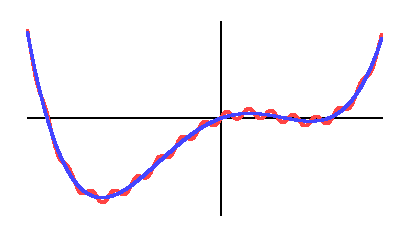
\includegraphics{consistency-error}\end{center}
Assume that our code for evaluating~$f$ actually evaluates the function given
by the red curve. If we are only interested in the function values, we might be
content with this approximation. However, automatic differentiation would yield
the derivative of the red curve, which is far off from the derivative of~$f$.
One could describe such a situation as ``discretize first, then
derive'' instead of ``derive first, then discretize''.

Fortunately, this kind of pathology doesn't seem to occur often in real world
problems. Give it a try!

\paragraph{Synthetic differential geometry} Do you want to employ infinitesimal
numbers like~$\varepsilon$ not only in your numerical algorithms, but also in
your theoretical mathematical research? Do you want to freely
use~$\varepsilon$'s as the physicists do? There is a way to do that, while at
the same time staying mathematically rigorous. Check out an expository
blog post by Andrej Bauer

\begin{center}\small\url{http://math.andrej.com/2008/08/13/intuitionistic-mathematics-for-physics/comment-page-1/}\end{center}

or these notes for high school students (in German):

\begin{center}\small\url{https://github.com/iblech/mathezirkel-kurs/raw/master/thema05-sdg/blatt05.pdf}\end{center}

\end{document}
